\documentclass[a4paper,12pt]{article}
\usepackage{graphicx} 
\usepackage{amsmath} 
\usepackage{amssymb} 
\usepackage{geometry} 
\usepackage{fancyhdr} % for headers and footers
\usepackage{caption} % for customizing captions
\usepackage{subcaption}
\usepackage{setspace} 
\usepackage[bottom]{footmisc}
\usepackage{adjustbox}
\usepackage{placeins}
\usepackage{float}
\usepackage{wrapfig}
\usepackage[nopatch=item]{microtype}
\usepackage{enumitem} % for customizing lists
\usepackage[backend=biber]{biblatex} % for bibliography
\usepackage[colorlinks,linkcolor=blue,citecolor=blue,urlcolor=blue]{hyperref}
%\addbibresource{Sci. Data_01.bib} % specify your bibliography file

\setlength{\parindent}{1.27cm} % Indent first line of each paragraph by 1.27 cm (0.5 inches)

\geometry{margin=1in}
\setlength{\parindent}{0pt}
\setlength{\parskip}{6pt}
\doublespacing

 
\pagestyle{fancy}
\fancyhf{}
\fancyhead[L]{\leftmark}
\fancyfoot[C]{\thepage}

\begin{document}

\begin{wrapfigure}{l}{0.25\textwidth} % 'r' indica destra, '0.3\textwidth' la larghezza
    
\includegraphics[width=\linewidth]{THE.png}
    \vspace{-25pt}
\end{wrapfigure}
 Fourier transform is the most widely used tools in applied mathematics
to analyze signals. The essence of the Fourier transform of a waveform is to decompose
or separate the waveform into a sum of sinusoids of different frequencies.
If these sinusoids sum to the original waveform, then we have determined
the Fourier transform of the waveform.
Mathematically speaking, is it possible to write this relation as:
$$
\mathcal{S}(f) = \int_{-\infty}^{+\infty} s(t) e^{i2\pi f t} dt,
$$
where s(t) is the waveform to be decomposed into a sum of sinusoids
and $\mathcal{S}(f)$ is the Fourier transform of s(t).
As an example, consider the
pulse waveform (\ref{fig:pulse}) and its Fourier transform (\ref{fig:fourier_pulse}) shown the following figures.
\begin{figure}[H]
    \centering
    % First row with two images
    \begin{minipage}[b]{0.40\linewidth} % 45% of line width for the first image
        \centering
        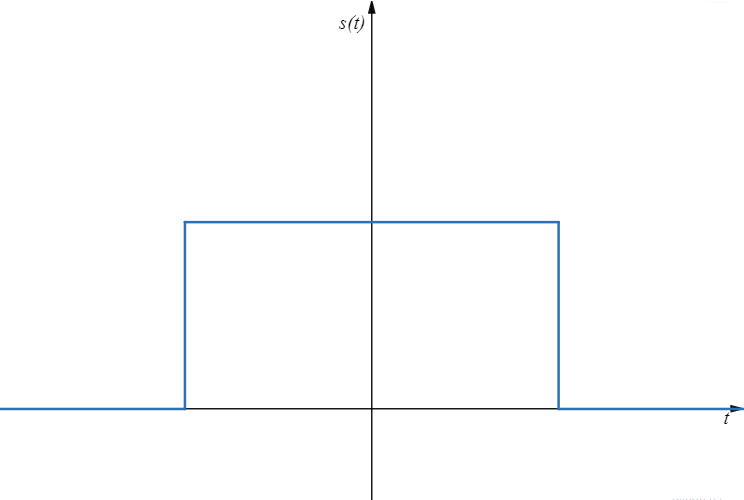
\includegraphics[width=\linewidth]{pulse.png}
        \caption{pulse waveform}
        \label{fig:pulse}
    \end{minipage}
    \hspace{0.05\linewidth} % Small horizontal space between images
    \begin{minipage}[b]{0.40\linewidth} % 45% of line width for the second image
        \centering
        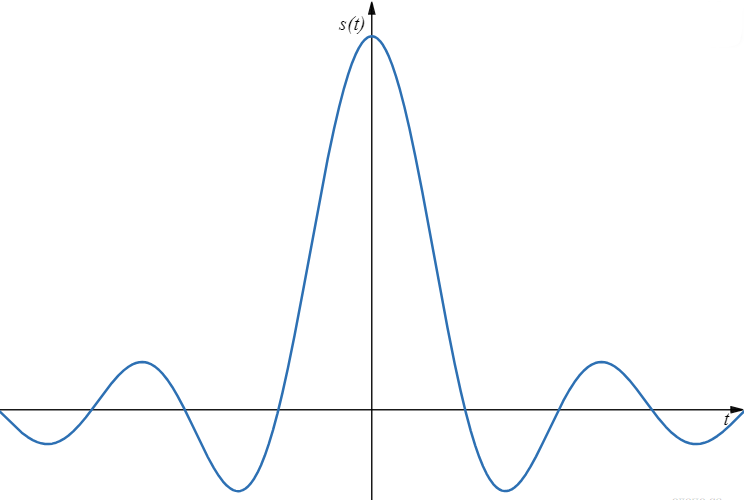
\includegraphics[width=\linewidth]{f.t_pulse.png}
        \caption{Fourier transform }
        \label{fig:fourier_pulse}
    \end{minipage}
\end{figure}
The Fourier transform is a powerful tool for signal analysis and is also highly 
effective for reducing noise within a signal. In this experiment, we analyze a
sinusoidal signal affected by noise, where the noise is represented as a set of 
discrete random variables that are uncorrelated, have zero mean and 
finite variance. Given this, we apply the square root law, anticipating that 
the standard deviation of the mean will decrease proportionally with the square 
root of the number of acquisitions.
Thus, the primary goals of this experiment are: first, to demonstrate 
that we can use the Fourier transform to reduce noise and obtain a cleaner 
signal, and second, to verify that the standard deviation of the mean indeed 
decreases as predicted by the square root of the number of acquisitions.



\section{Materials and Methods}
\subsection{Equipment And Tools}
\begin{itemize}
    \item Digital storage oscilloscope (Siglent - SDS5034X)
    \item Waveform generator (Siglent - SDG6022X)
    \item Two BNC-to-BNC cables
    \item USB flash drive
\end{itemize}

\subsection{Experimental Procedure}
We started by connecting the digital oscilloscope to the waveform generator 
using BNC-to-BNC cables. Then, we proceeded to generate a sinusoidal signal 
with a frequency of 1 kHz and an amplitude of 2 Vpp, along with a noise signal, 
using the waveform generator.
Next, using a function of the digital oscilloscope, we were able to add the two signals.
The resulting waveform can be seen in the following figures. 

\begin{figure}[H]
    \centering
    % First row with two images
    \begin{minipage}[b]{0.40\linewidth} % 45% of line width for the first image
        \centering
        \label{fig:sin}
        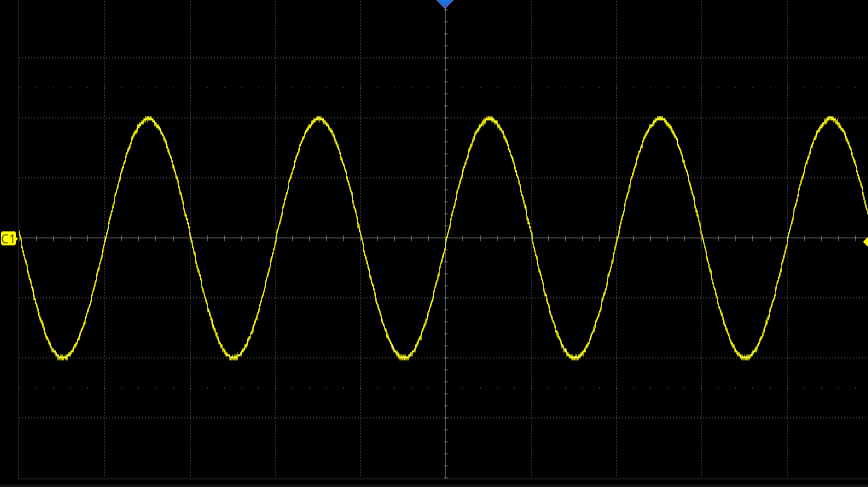
\includegraphics[width=\linewidth]{sin.png}
        \caption{Sinusoidal signal}
    \end{minipage}
    \hspace{0.05\linewidth} % Small horizontal space between images
    \begin{minipage}[b]{0.40\linewidth} % 45% of line width for the second image
        \centering
        \label{fig:noise}
        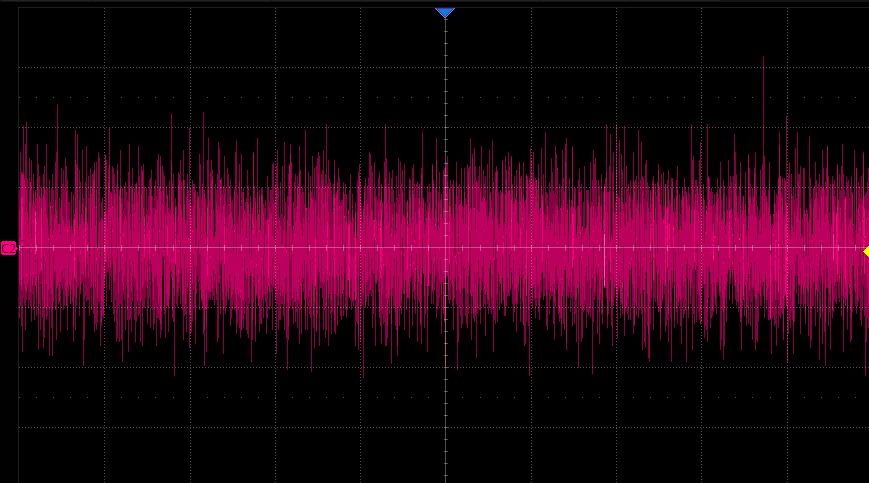
\includegraphics[width=\linewidth]{noise.png}
        \caption{Noise signal}
    \end{minipage}
    
    % Second row with centered image
    \vspace{0.5cm} % Vertical space between rows
    \begin{minipage}[b]{0.40\linewidth} % 60% of line width for the third image
        \centering
        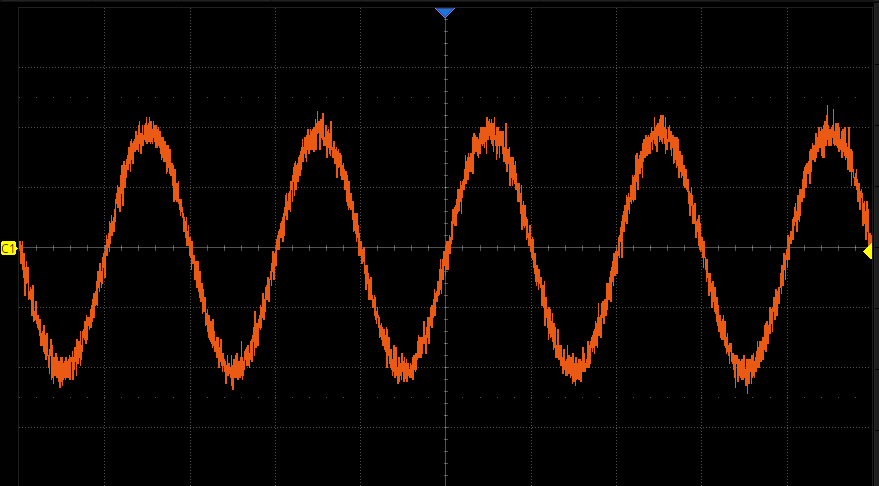
\includegraphics[width=\linewidth]{noise_signal.png}
        \label{fig:sin+noise_signal}
        \caption{Resulting signal from the addition of the two signals} 
    \end{minipage}
    
\end{figure}
Finally, we proceeded to acquire the data from the oscilloscope and saved it to a USB flash drive.
To acquire the data from the oscilloscope, we followed the steps below:
\begin{itemize}
    \item press the save/recall button, to open the file acquisitions menu
    \item select the the file extension, in our case .csv
    \item select our USB flash drive from the acquisition menu
    \item press on the touch screen the save as window
    \item select the file name and press the save button
\end{itemize}
All the data acquired was analyzed using Julia programming language 
% \cite{}. mettere su e aggingere la citazione al sito di julia https://julialang.org/
 






\end{document}